\chapter[Introduction: Radio and Pulsars]{Introduction to Radio Wavelength Emission Physics and Modeling of Pulsar Magnetospheres}
\label{chapter:radioAndPulsars}
In this chapter we will explore in more depth the physical models of the pulsar magnetosphere and 
physical phenomena highly relevant to fully understanding
the observed emission.  The focus here is
on analytic models derived elsewhere and 
standard to the current understanding
of pulsar magnetospheres.  
We will discuss further the numerical models of pulsars
utilized in this thesis in Chapter \ref{chapter:numericalModels}. 

\section{Polarization}
\label{sec:polarization}

William Hilter and John Hall first observed polarization of starlight in 1949 \citep{hiltner1949polarization,hall1949observations}.
Polarization was soon linked to magnetic fields of the galaxy 
by Leverrett Davis, Jr. and Jesse Greenstein \citep{davis1951polarization}.

Pulsars have strong magnetic fields which gives rise to not only their 
extremely focused beam of emission but also coherent light with 
defined polarization.  
Polarization is a means of observing the magnetic field lines of these incredibly small,
far away objects.  That we can make such a bold measurement speaks to the extremes of the
pulsar.


Polarization is most often reported in terms of Stokes parameters, $I$, $Q$, $U$, and $V$.
Stokes parameters are a standard way of representing polarization.
At a radio telescope with polarization measurement capabilities, the incoming
electromagnetic wave is converted to electric voltage in two independent
feeds.  Linear feeds will measure polarization aligned along $x$ and $y$ Cartesian coordinates
while circular feeds will measure polarization as right-handed or left-handed.

Components of the linear and circular feeds can be converted to Stokes parameters
\begin{equation}
 \begin{array}{lcl}
    I=\langle E_{\rm X}^{2} \rangle + \langle E_{\rm Y}^{2} \rangle &\textrm{and}& I=\langle E_{\rm R}^{2} \rangle + \langle E_{\rm L}^{2} \rangle,\\
    Q=\langle E_{\rm X}^{2} \rangle - \langle E_{\rm Y}^{2} \rangle &\textrm{and}& Q=2\langle E_{\rm R}^{2} E_{\rm L}^{2} \cos {\left(\kappa_{\rm RL}\right)} \rangle,\\
    U=2\langle E_{\rm R}^{2} E_{\rm L}^{2} \cos {\left(\kappa_{\rm XY}\right)} \rangle &\textrm{and}& U=2\langle E_{\rm R}^{2} E_{\rm L}^{2} \sin {\left(\kappa_{\rm RL}\right)} \rangle,\\
    V=2\langle E_{\rm R}^{2} E_{\rm L}^{2} \sin {\left(\kappa_{\rm XY}\right)} \rangle &\textrm{and}& V=\langle E_{\rm R}^{2} \rangle - \langle E_{\rm L}^{2} \rangle,
  \end{array}
\end{equation}
where $\kappa_{\rm AB}$ is the phase difference.
With a little manipulation, we can see that $I^2=Q^2+U^2+V^2$ if the incoming signal is
totally polarized.  Typically, $(Ip)^2=Q^2+U^2+V^2$, where $p$ is the degree of polarization.

\begin{figure}[h]
\vskip .42\textheight
\begin{center}
%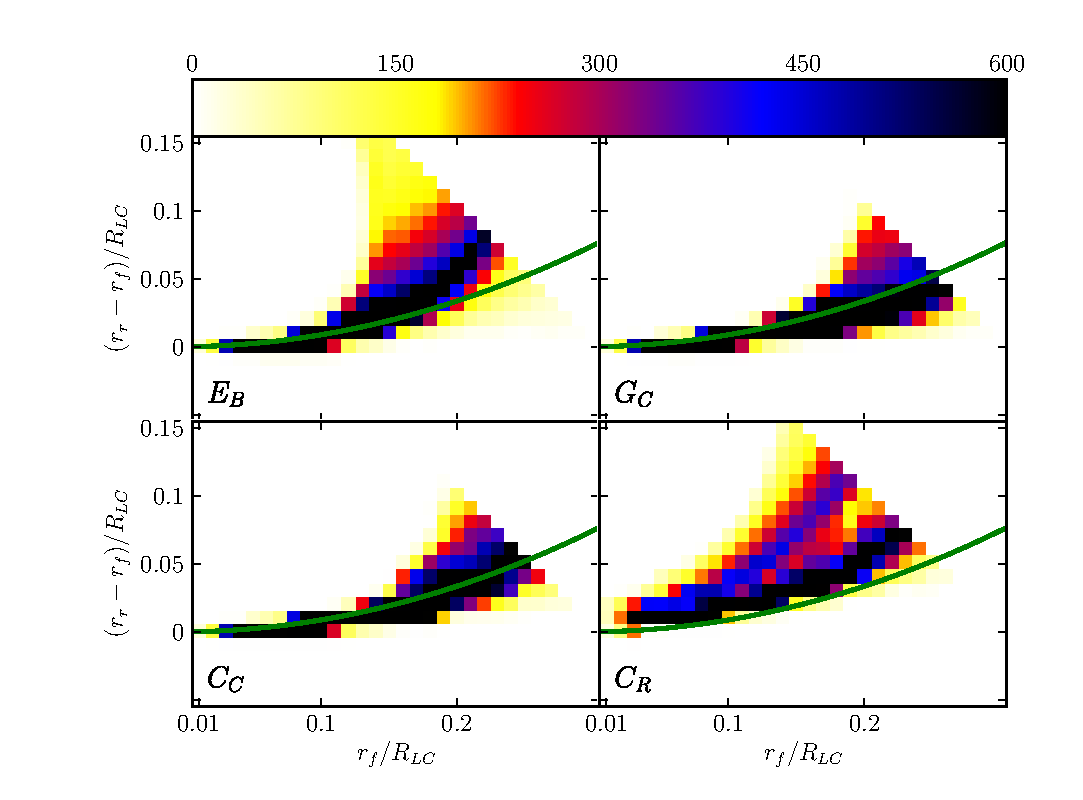
\includegraphics[width=.7\textwidth]{chapter2figures/totDirFitPhi.eps}
\special{psfile=chapters/radioDataAnalyticModels/figures/stokesFigure.eps hoffset=-100 voffset=-300 vscale=100 hscale=100}
\caption[Visualization of Stokes parameters]{
Visualization of Stokes parameters.  The absolute value of linear polarization ($|L|=\sqrt{U^2+Q^2}$ )
occupies the $U$-$Q$ plane while circular polarization $V$ is the third Cartesian axis.  The
total polarized intensity is labeled $pI$ and the total intensity which extends beyond
the polarized intensity is labeled $I$.
}
\label{fig:stokes}
\end{center}
\vskip -.03\textheight
\end{figure}

Stokes parameters are a convenient way of expressing polarization and is particularly useful for
describing partially polarized light using $p$. The Stokes parameters occupy the so-called
Poincar\'{e} sphere of optics where $Q$, $U$, and $V$ are the axes and $pI$ is the radius of the
sphere (Figure~\ref{fig:stokes}).  The polarization angle ($\psi$) and linear polarization ($L$) relate to the polar coordinates of
$Q$ and $U$:

\begin{equation}
    |L|=\sqrt{U^2+Q^2}
\end{equation}
\begin{center}
and
\end{center}
\begin{equation}
    \psi=\frac{1}{2} \arctan{\left(\frac{U}{Q}\right)}.
\end{equation}

Polarization data that we received from collaborators is in the form
of $Q$, $U$, $V$, $I$ versus pulsar rotation period phase and we
calculate polarization using $Q$ and $U$.

Further error bars for the polarization are calculated using the
following formula (standard error propagation):

\begin{equation}\sigma_{\psi}(\phi)=\frac{1}{2} \frac{\sqrt{\langle\sigma_{U{\rm off}}*Q(\phi)\rangle^2+\langle\sigma_{Q{\rm off}}*U(\phi)\rangle^2}}{\langle Q(\phi)\rangle^2+\langle U(\phi)\rangle^2}.\end{equation}

The values $\sigma_{Q{\rm off}}$ and $\sigma_{U{\rm off}}$ are the standard deviation in the off-pulse phases of $Q$ and $U$.
Note that $Q$, $U$, and $\sigma_{\psi}$ are all functions of the 
pulsar rotation period phase, $\phi$.


\section{Effects of Interstellar Medium} \label{sec:interstellarScattering}
The space between us and pulsars is not empty but is full
of ionized medium that effects electromagnetic waves.
Such medium modifies the signal in several ways which we can
quantify.

The dispersion measure is the total density of free electrons ($N(l)$) over the intervening space that the signal from the pulsar
travels:
\begin{equation} DM=\int_0^L N(l) \mathrm{d}l. \end{equation}

The dispersion measure is related to the frequency of the emission ($\nu$) and the time delay of the emission ($t$):

\begin{equation}DM_{[\textrm{cm}^{-3}\textrm{pc}]}=2.410\times10^{-4} \textrm{ } t_{[\textrm{s}]}\textrm{ } \nu^2_{[\textrm{MHz}]}.\end{equation}

This formula is useful for calculating the expected time delay between frequencies:

\begin{equation}
\Delta t_{[\textrm{s}]}= \frac{DM_{[\textrm{cm}^{-3}\textrm{pc}]}}{2.410\times 10^{-4}} \left\{  \frac{1}{\nu^2_{2 [\textrm{MHz}]}} - \frac{1}{\nu^2_{1 \lbrack\textrm{MHz}\rbrack}}  \right\}.\end{equation}

In particular, we wished to quantify the time delay in PSR J1420$-$6048 because the fit was simultaneous
in two frequencies, 10cm and 20cm (Section \ref{sec:J1420}).  
In the end, we found that any time delay due to dispersion
was overpowered by our uncertainty in phase. (See \cite{rohlfs2000tools} for a particularly well formulated
presentation of the dispersion measurement calculation.)

Another effect of interstellar medium on measurements is interstellar scattering.
The scattering of emission in the medium results in multipath propagation.  
The effects of interstellar scattering manifest themselves in pulsar data as
a broadening of the trailing end of the intensity pulse and a flattening of the polarization data versus
phase.

This scattering effect is mathematically described as a convolution of the unscattered
Stokes parameters with a scattering kernel:

\begin{equation}
\begin{array}{l}
I^{\rm scat}=\int I(\phi(t')) g(t-t') dt,\\
Q^{\rm scat}=\int Q(\phi(t')) g(t-t') dt,\\
U^{\rm scat}=\int U(\phi(t')) g(t-t') dt,\\
V^{\rm scat}=\int V(\phi(t')) g(t-t') dt.
\end{array}
\end{equation}
This relation is used for model $Q$ and $U$
in Chapter \ref{chapter:tacklingPolarization}.

Analytical scattering kernels exist assuming various distributions
of interstellar medium.  
The scattering kernel assuming a thin scattering screen 
halfway between source and observer is given by 

\begin{equation}\label{eq:gts2}
g_{ts}(t-t')=\left\{
\begin{array}{lr}
0,                       & t-t' < 0 \\
e^{-(t-t') / \tau_{\rm s}},  & t-t' > 0
\end{array}
\right.
\end{equation}
\citep{williamson1972pulse,williamson1973pulse}.
The scattering kernel assuming a thick screen near the
source is given by 
\begin{equation}
g_{\rm ths}(t-t')=\left\{
\begin{array}{lr}
0,                       & t-t' < 0 \\
\sqrt{\frac{\pi \tau_{\rm s}}{4t^3}} e^{-\pi^2\tau_{\rm s}/16t},  & t-t' > 0.
\end{array}
\right.
\end{equation}
The scattering kernel assuming uniform medium is given by
\begin{equation}
g_{\rm um}(t-t')=\left\{
\begin{array}{lr}
0,                       & t-t' < 0 \\
\sqrt{\frac{\pi^5 \tau_{\rm s}^3}{8t^5}} e^{-\pi^2\tau_{\rm s}/4t},  & t-t' > 0.
\end{array}
\right.
\end{equation}
The variable $\tau_{\rm s}$ is a characteristic scattering time.
The simplest kernel $g_{\rm ts}$ is used in Chapter \ref{chapter:tacklingPolarization}  in 
modeling scattering.

Finally, pulsar polarization data is Faraday rotated
by interstellar medium.  Faraday rotation is a powerful
tool for probing interstellar scattering but for us it is 
a nuisance to be removed from the data.  The degree of Faraday rotation
is related to frequency and can be removed by comparing data
from multiple frequencies.  Considering that $\Delta\psi$ is often
treated as a nuisance parameter, the accuracy of this removal
is not very important.  



\section{Beaming Geometry}
\label{sec:beamingGeometry}
Assuming a beam of emission centered on the 
magnetic axis, the
relationship between pulse width
in phase and the opening angle of the
cone structure where emission originates
can be derived in closed form.
The cone is centered on the magnetic 
axis defined by 

\begin{equation}
\label{equ:m}
\hat{m}=\cos{(\phi)} \sin{(\alpha)} \hat{x} + \sin{(\phi)} \sin{(\alpha)} \hat{y} + \cos{(\alpha)} \hat{z}
\end{equation}
where $\phi$ is the phase of the pulsar
as it rotates about $\hat{\Omega}=\hat{z}$.
The pulse width is $W$ and thus
for a symmetric cone, the 
pulse is seen between $\phi=-W/2$ and $\phi=W/2$
in phase.
The angle between $\hat{m}$ and the
line of sight at the maximums ($\phi=-W/2$ and $\phi=W/2$) will also be the opening
angle.  The line of sight is given by 
\begin{equation}
\hat{n}=\sin{\zeta} \hat{x}+\cos{\zeta} \hat{z}
\end{equation}
and the relation between opening angle and 
pulse width is
\begin{equation}
\label{equ:ndotm}
\hat{n}\cdot\hat{m}=\cos{\Gamma}=\sin{\zeta} \cos{W/2} \sin{\alpha} + \cos{\zeta} \cos{\alpha} 
.\end{equation}
This equation makes no assumptions about the form of the magnetic field lines.
The angle $\alpha$ is between the spin axis and the magnetic axis and the
angle $\zeta$ is between the spin axis and the line of sight.

We can further relate the pulse width to emission height for a
dipole magnetic field.  The last closed field lines
which define the emission cone for a simple dipole
have the form 
\begin{equation}
\label{equ:dipole}
\mathbf{r}=\sin^3\theta \hat{x} + \sin^2\theta \cos{\theta} \hat{z}
\end{equation}
\begin{center}
and
\end{center}
\begin{equation}
R=|\mathbf{r}|=\sin^2\theta
\end{equation}
in polar coordinates where $R$ is the emission 
altitude measured in $R_{\rm LC}$, light cylinder
radius.
In this coordinate system, $\hat{m}=\hat{z}$.

The angle $\Gamma$ between $\hat{n}$ and $\hat{m}$
will be approximately the angle between 
\begin{equation}
\hat{T}=\frac{d\mathbf{r}/d\theta}{|d\mathbf{r}/d\theta|}
\end{equation}
(the curvature of $\mathbf{r}$) and $\hat{m}$.
This is actually a far field approximation 
but is appropriate because 
the observer is very far from the pulsar.

We can then relate the opening
angle to the altitude using Equation \ref{equ:dipole}.
Again using $\hat{m}=\hat{z}$, Equation \ref{equ:dipole} and Equation \ref{equ:m}:
\begin{equation}\hat{T}\cdot\hat{m}=\frac{2-3\sin^2\theta}{\sqrt{4-3\sin^2\theta}}.\end{equation}

Using $R=\sin^2\theta$ and approximating $R$ as small, 
\begin{equation}\hat{T}\cdot\hat{m}=1-9R/8.\end{equation}

Further using $\hat{T}\cdot\hat{m}\approx\cos{\Gamma}\approx 1-\Gamma^2/2$ and Equation \ref{equ:ndotm},
we get:
\begin{equation}
R=\frac{4}{9}\arccos^2\left[\sin{\zeta}\cos{\frac{W}{2}}\sin{\alpha}+\cos{\zeta}\cos{\alpha}\right]
.
\end{equation}

This equation then relates the width of the intensity pulse to the altitude of
emission.

\section{Rotating Vector Model}
\label{sec:RVMformula}

The rotating vector model (RVM) relates the 
geometrical angles $\alpha$ (the angle between
the spin axis and the magnetic axis) and $\zeta$ (the
angle between the spin axis and the line of sight)
to the polarization position angle $\psi$ for 
a given phase angle $\phi$.

We start with a fixed magnetic axis given by
\begin{equation}
\hat{m}=\sin{\alpha}\hat{x}+\cos{\alpha}\hat{z}
\end{equation}
and a viewing direction given by
\begin{equation}
\hat{n}=\sin{\zeta}\cos{\phi}\hat{x}+\sin{\zeta}\sin{\phi}\hat{y}+\cos{\zeta}\hat{z}.
\end{equation}
The polarization angle with respect to $\hat{z}=\vec{\Omega}$
is the difference in angle between the projection of $\hat{z}$
onto the viewing plain and the projection of the vector 
$\hat{n}-\hat{m}/|\hat{n}-\hat{m}|$.
The viewing plane is defined as orthogonal to $\hat{n}$.
These projections can then be given by the vector rejections:
\begin{equation}
\mathbf{P}_{\Omega}=\mathbf{\hat{z}}-(\mathbf{\hat{z}}\cdot\mathbf{\hat{n}})\mathbf{\hat{n}}
\end{equation}
and 
\begin{equation}
\mathbf{P}_{m-n}=\frac{\hat{n}-\hat{m}}{|\hat{n}-\hat{m}|}-\left(\frac{\hat{n}-\hat{m}}{|\hat{n}-\hat{m}|}\cdot\mathbf{\hat{n}}\right)\mathbf{\hat{n}}
.\end{equation}

The polarization angle can be calculated as
\begin{equation}
\tan{\psi}=\frac{|\mathbf{P}_{m-n}\times\mathbf{P}_{\Omega}|}{\mathbf{P}_{m-n}\cdot\mathbf{P}_{\Omega}}
.\end{equation}

Plugging in the above formulas and simplifying gives us the familiar 
rotating vector model equation:
\begin{equation}
\tan{\psi}=\frac{
-\sin{\alpha}\sin{\phi}
}{
\cos{\alpha}\sin{\zeta}-\cos{\phi}\cos{\zeta}\sin{\alpha}
}
.\end{equation}


